\begin{frame}{Observing von Kármán Vortex Street}
    \textbf{Setup:}
    \begin{itemize}
        \item Flow with $\Rey = 500$ ($ \Leftrightarrow\, U = 0.03012$).
        \item Simulation domain: $\dd{x} = \dd{y} = 0.01 $ with a $500 \times 100$ grid.
        \item Circular obstacle with radius $r = 0.125$ initiates flow.
    \end{itemize}
    \vspace{-0.25cm}
    \begin{figure}
        \centering
        \hspace*{0.3cm}
        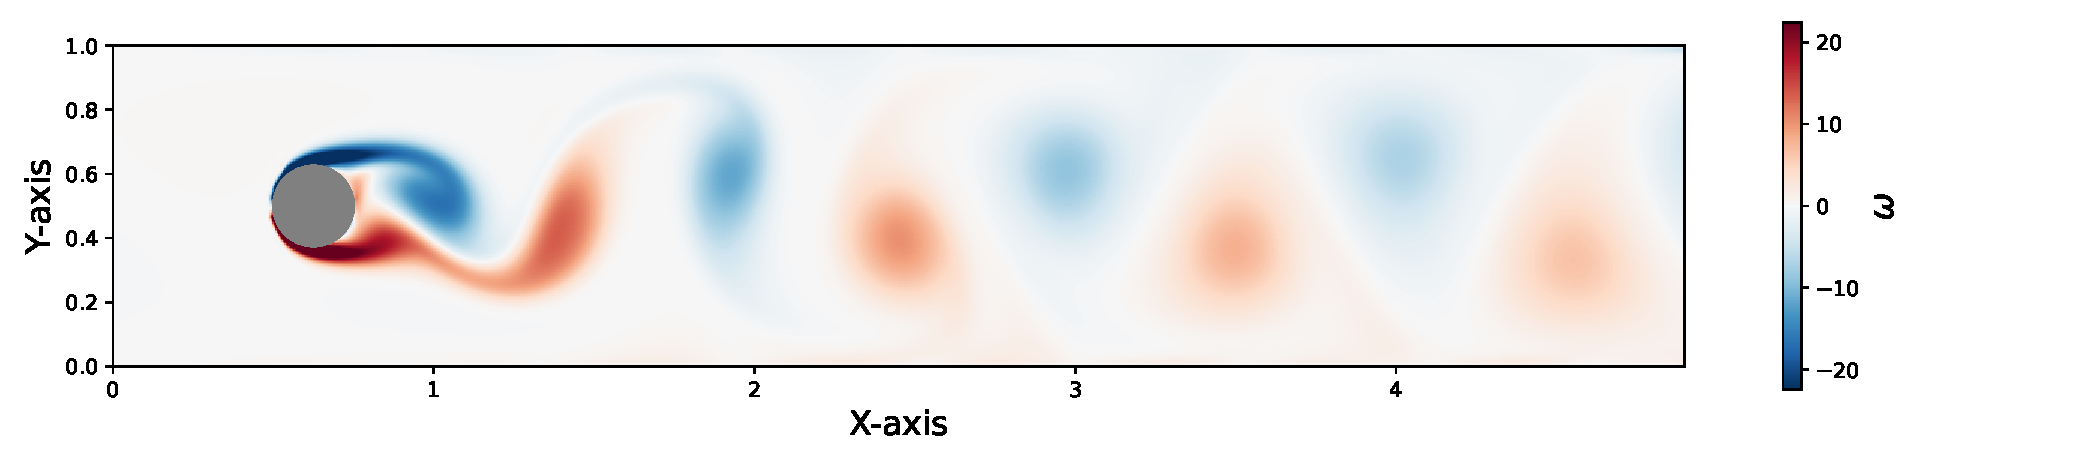
\includegraphics[width=1.1\linewidth]{graphics/numeric/vor_25_sim.pdf}
        \caption{Vorticity $\omega = \nabla \times \vf{u}$ highlighting alternating vortices}
        \label{fig: first_obs}
    \end{figure}
    \vspace{-0.25cm}
    \textbf{Obervations:}
    \begin{itemize}
        \item Laminar front with $u = 1$
        \item Von Kármán vortex street and periodic pattern formation
    \end{itemize}
\end{frame}

\begin{frame}{Influence of Reynolds Number on Flow Dynamics}
    \begin{itemize}
        \item The Reynolds number dictates flow behavior in fluid dynamics.
        \item At a critical $\Rey \approx 175$, flow transitions from laminar to unstable, eventually forming a von Kármán vortex street.
    \end{itemize}
    \vspace{-0.25cm}
        
    \begin{figure}
        \centering
        \hspace*{0.3cm}
        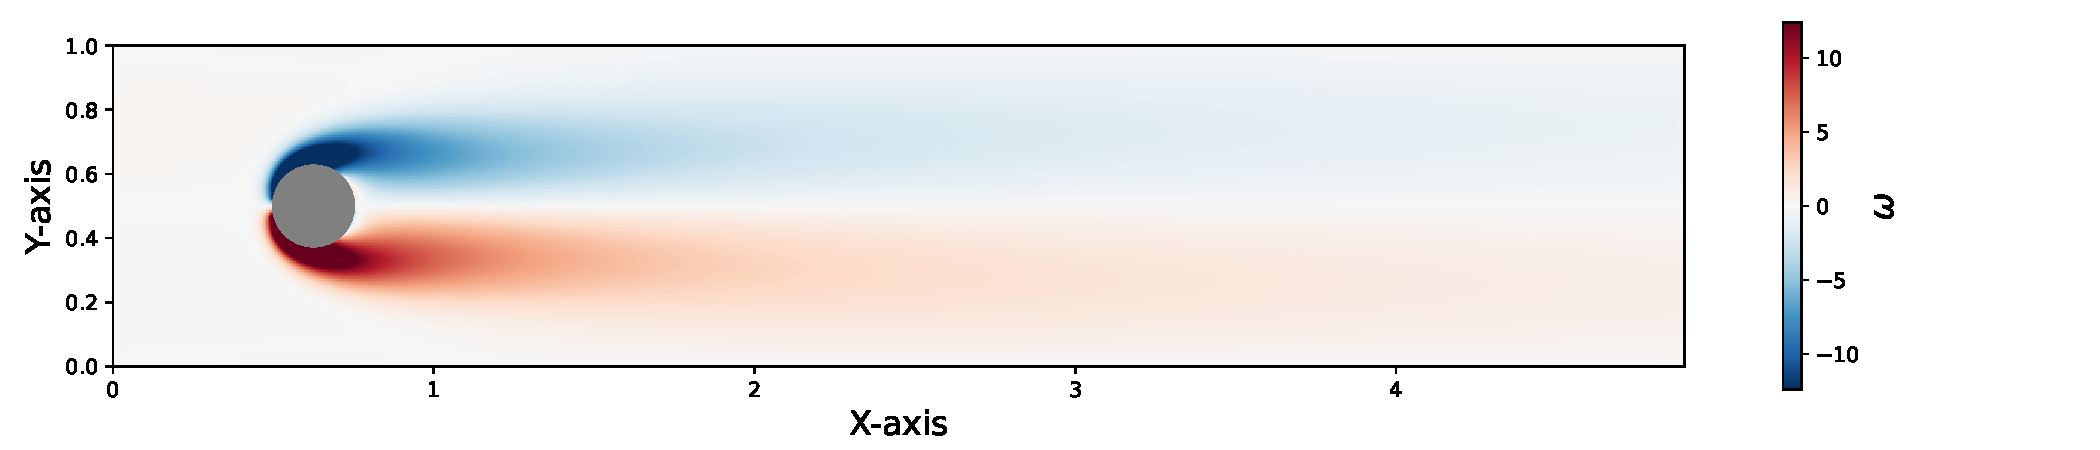
\includegraphics[width=1.1\linewidth]{graphics/numeric/RE100_30_sim.pdf} % Update path accordingly
        \vspace{-0.7cm}
        \caption{Laminar flow at $\Rey = 100$ ($ \Leftrightarrow\, U = 0.006$)}
    \end{figure}
    \vspace{-0.7cm}
    \begin{figure}
        \centering
        \hspace*{0.3cm}
        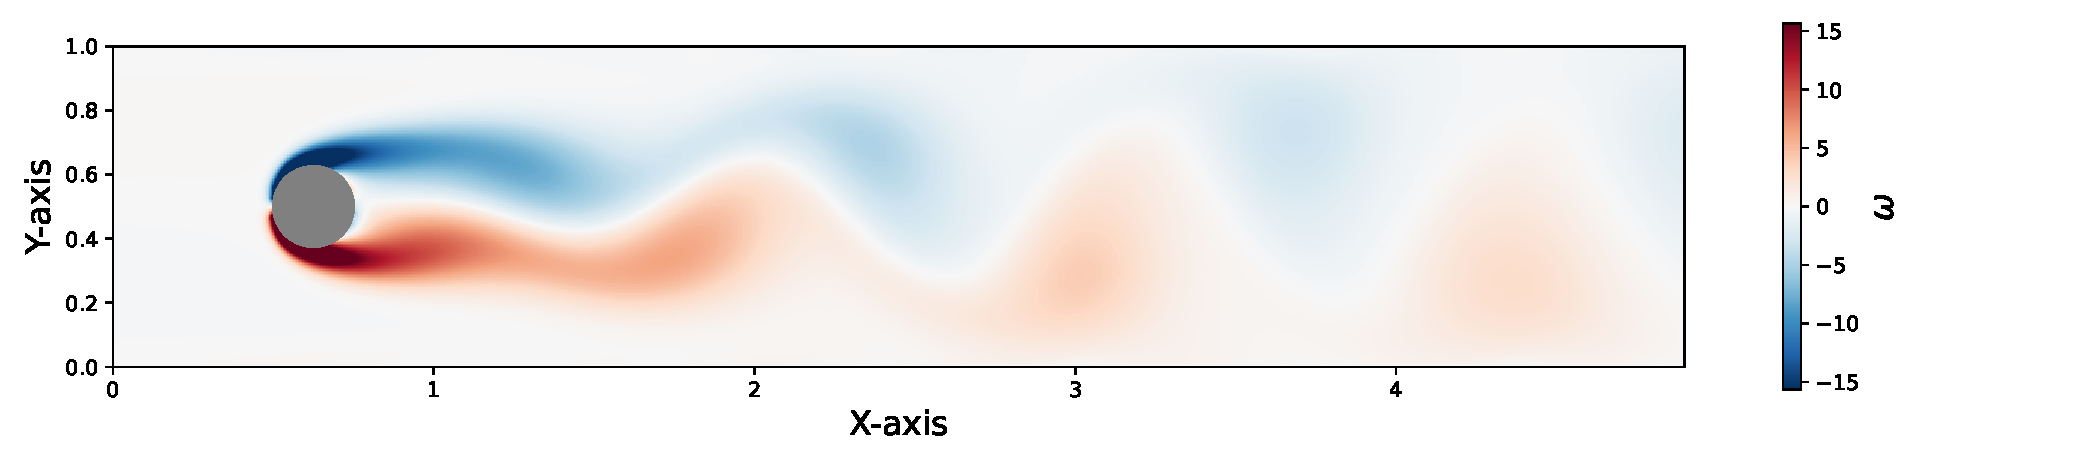
\includegraphics[width=1.1\linewidth]{graphics/numeric/RE190_30_sim.pdf} % Update path accordingly
        \vspace{-0.7cm}
        \caption{Vortex street at critical $\Rey = 190$ ($ \Leftrightarrow\, U = 0.0114$)}
    \end{figure}

\end{frame}

\begin{frame}{Influence of the shape on the flow}
    \begin{figure}
        \centering
        \hspace*{0.3cm}
        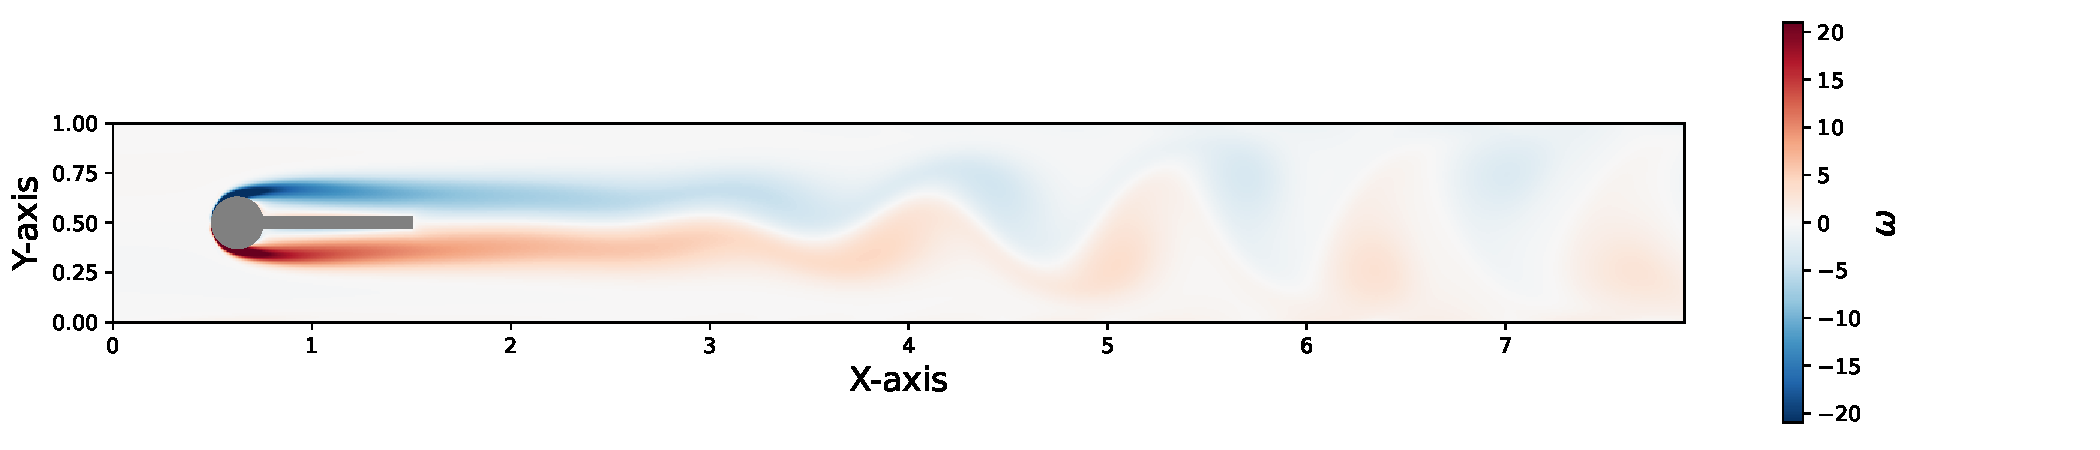
\includegraphics[width=1.1\linewidth]{graphics/numeric/vor_30_circlefin.pdf}
        \vspace{-0.7cm}
        \caption{Flow around circle with fin at $\Rey = 500$ ($ \Leftrightarrow\, U = 0.03012$)}
    \end{figure}
    \textbf{Observation:}
    \begin{itemize}
        \item Fin alters flow, delaying the separation.
        \item Flow transitions at $\Rey \approx 500$, enhancing mixing and vortex complexity.    
    \end{itemize}
\end{frame}

\begin{frame}{Optimized shape: Airfoil}
    %the wing to showcase the influence of the shape
    
    \begin{figure}
        \centering
        \hspace*{0.3cm}
        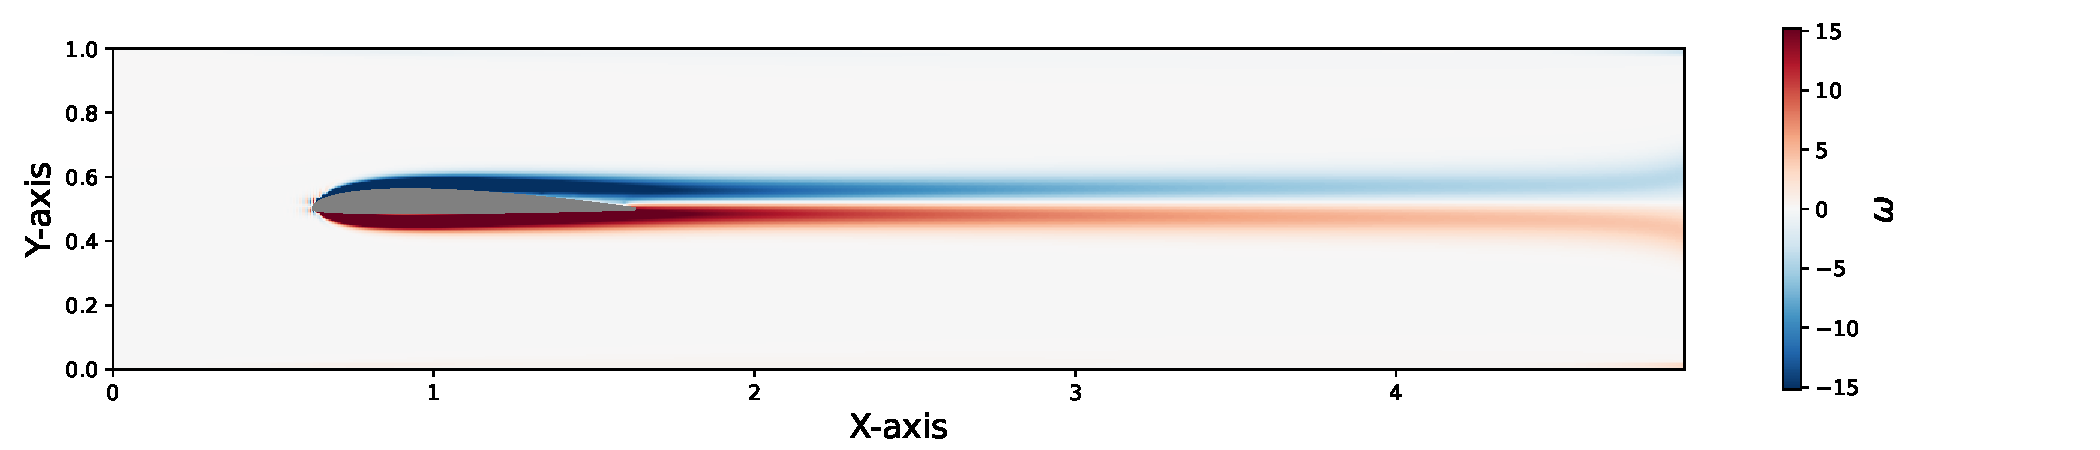
\includegraphics[width=1.1\linewidth]{graphics/numeric/RE3500_30_airfoil.pdf} % Update path accordingly
        \vspace{-0.7cm}
        \caption{Flow with airfoil at $\Rey = 500$ ($ \Leftrightarrow\, U = 0.1076$)}
    \end{figure}
    \vspace{-0.7cm}
    \begin{figure}
        \centering
        \hspace*{0.3cm}
        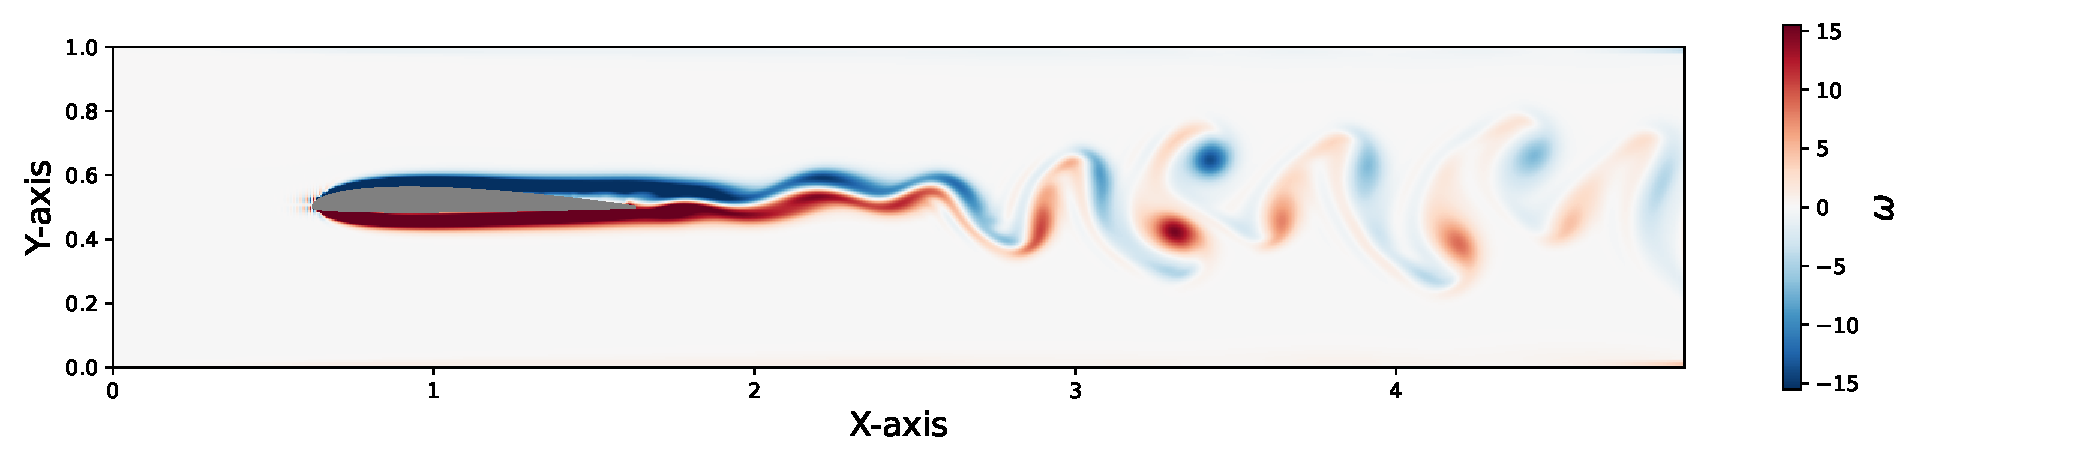
\includegraphics[width=1.1\linewidth]{graphics/numeric/RE5500_30_airfoil.pdf} % Update path accordingly
        \vspace{-0.7cm}
        \caption{Flow with airfoil at $\Rey = 5500$ ($ \Leftrightarrow\, U = 1.1833$)}
    \end{figure}
    \vspace{-0.3cm}
    \textbf{Key Insight:} Airfoil shape minimizes vortex shedding. Streamlined design reduces flow separation and turbulence at higher speeds.
\end{frame}